% !TeX root = ../project.tex

\section{Design decisions}
During the sketching phase, several design choices were discussed. One of the very first decisions made was the overall look of the menu. The choice of big buttons, clear visual cues and short textual descriptions was present in almost all of the sketches in the early design phase, as seen in figure (HVILKEN FIGURE???):\\
\begin{figure}
\centering
  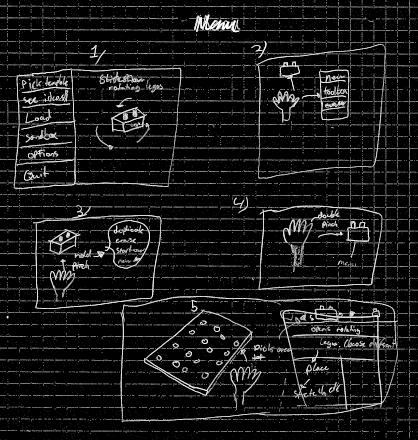
\includegraphics[width=0.9\columnwidth]{figures/Menu/menu2.png}
  \caption{Skriv lidt lækert her. }~\label{fig:genboard}
\end{figure}
\begin{figure}
\centering
  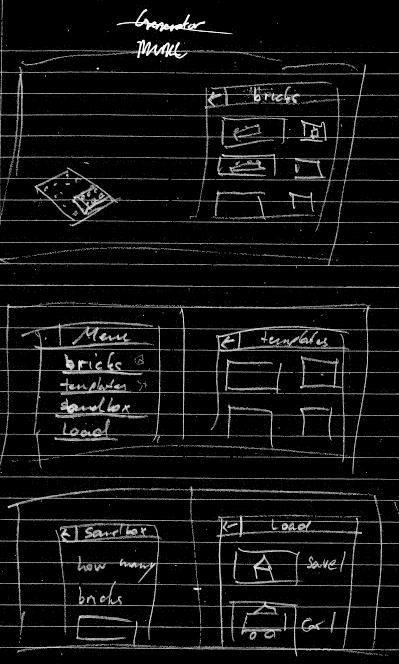
\includegraphics[width=0.6\columnwidth]{figures/Menu/menu1.png}
  \caption{Skriv lidt lækert her. }~\label{fig:genboard}
\end{figure}

\subsection{Suitability of LEGO in AR}
One of the aspects with the application was the suitability of LEGO in an AR setting. This question was asked rather late in the development process. What became apparent was that the virtual LEGO in an AR setting would not be able to provide the same "finicky" feel that LEGO has, sitting at a table, obsessing over small details in an advanced (?) setup. This is because of the computing limitiations of the Hololens and the technology architecture. The minimal rendering distance of the Hololens is, right now, much larger than the distance one would be from af real-life LEGO project, ie., arms length. This limitation demands a much larger brick size than real-life LEGO and this in turn limits the overall complexity of a virutal LEGO project. 